\subsection{Tarefa 5: Introdução de Ruído nos Dados de Treinamento}

\begin{comandoquestao}
Objetivo: Investigar como diferentes níveis de ruído nos dados de treinamento 
afetam a performance e a generalização da rede neural. Avaliaremos a robustez 
do modelo frente a dados ruidosos.
\end{comandoquestao}

Foram realizados experimentos de treinamento com quatro níveis diferentes de 
ruído adicionados aos dados: $\sigma=0.0$, $\sigma=0.1$, $\sigma=0.3$ e 
$\sigma=0.5$. O gráfico de treinamento para as diferentes redes é apresentada 
na \cref{fig:tarefas05:curvas}


\begin{figure}[tbh]
	\centering
	\caption{Curvas de aprendizado para diferentes níveis de ruído dos dados de 
	entrada}
	\label{fig:tarefas05:curvas}
	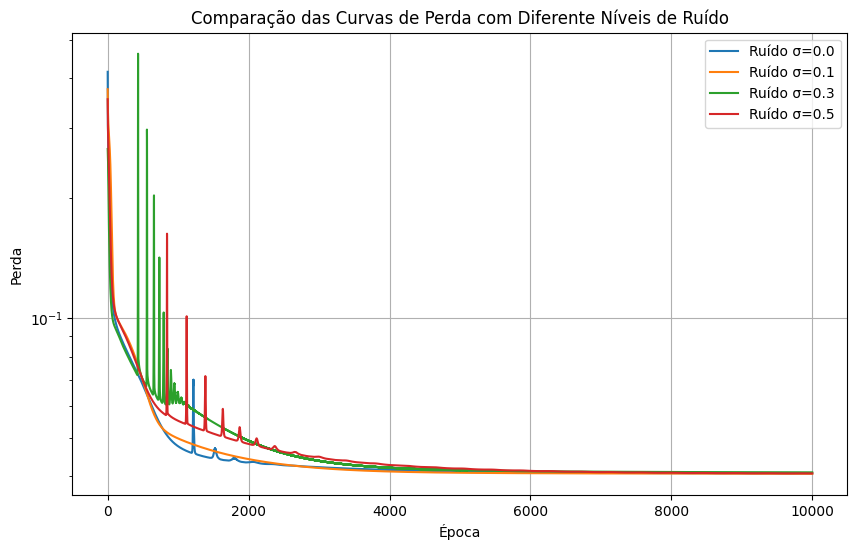
\includegraphics[width=0.7\linewidth]{./0803_imgs/0365_tarefa05/png-241110-193148800-7110775020035268662.png}
\end{figure}


Para $\sigma=\num{0,0}$, que 
representa dados sem ruído, os gráficos de perda 
mostram uma convergência suave e rápida, indicando que o modelo está aprendendo 
bem.

Para as redes com níveis de ruídos maiores, a convergência é ligeiramente mais 
lenta e a perda é um pouco maior em comparação com os dados sem ruído. Isso é 
esperado, pois o ruído adiciona complexidade aos dados, tornando a tarefa de 
aprendizagem mais desafiadora.

Com $\sigma=0,3$, a convergência torna-se mais instável, especialmente nas 
primeiras 
épocas do treinamento. A perda oscila mais e leva mais tempo para estabilizar. 
Isso sugere que o modelo está encontrando dificuldades para aprender os padrões 
subjacentes nos 
dados devido ao alto nível de ruído.

Para $\sigma=0,5$, é notável que a convergência parece 
mais estável do que $\sigma=0,3$ nas primeiras épocas, sugerindo que o modelo 
está encontrando maneiras de lidar com o ruído mais intenso. No entanto, como 
decorrer 
das épocas a taxa de erro volta a ficar maior que com o $\sigma=0,3$ como era 
esperado. 

A análise geral dos resultados revela uma relação interessante entre o nível de 
ruído e a convergência do modelo. Quanto maior o ruído, mais demorada é a 
convergência, o que é intuitivo, pois o modelo precisa lidar com mais incerteza 
nos dados. 
Apesar do ruído introduzido, pode-se ver nas 
\cref{fig:tarefa05:00:predicoes,fig:tarefa05:01:predicoes,fig:tarefa05:03:predicoes,fig:tarefa05:05:predicoes}
 que a predição das redes 
são adequadas.

\begin{figure}[htb]
	\centering
	\begin{minipage}{0.45\textwidth}
		\centering
		\caption{$\sigma=0.0$}\label{fig:tarefa05:00:predicoes}
		
		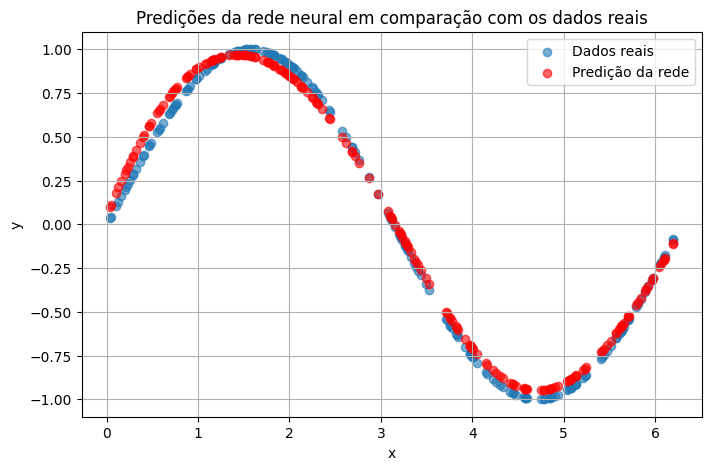
\includegraphics[width=\textwidth]{./0803_imgs/0365_tarefa05/png-241110-192904307-9336339325602212821.png}
		%\legend{Fonte: Gerado peloComando da atividade}
	\end{minipage}
	\hfill
	\begin{minipage}{0.45\textwidth}
		\centering
		\caption{$\sigma=0.1$}\label{fig:tarefa05:01:predicoes}
		
		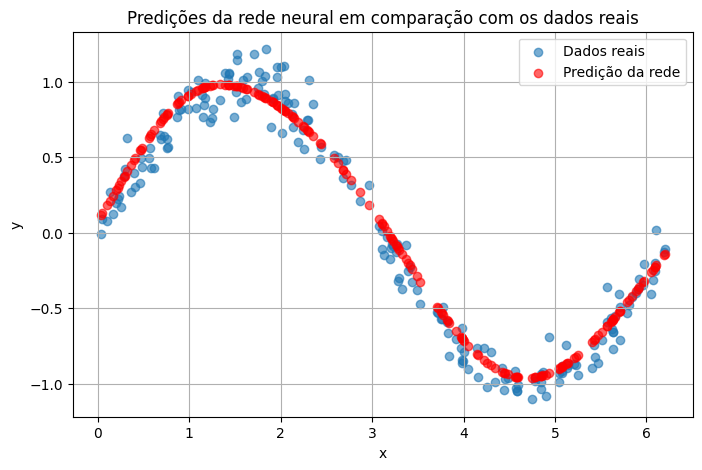
\includegraphics[width=\textwidth]{./0803_imgs/0365_tarefa05/png-241110-192925288-2928491021629715945.png}
		%\legend{Fonte: \citeonline[p. 24]{araujo2012}}
	\end{minipage}
	\vspace{2Ex}
	\begin{minipage}{0.45\textwidth}
		\centering
		\caption{$\sigma=0.3$}\label{fig:tarefa05:03:predicoes}
		
		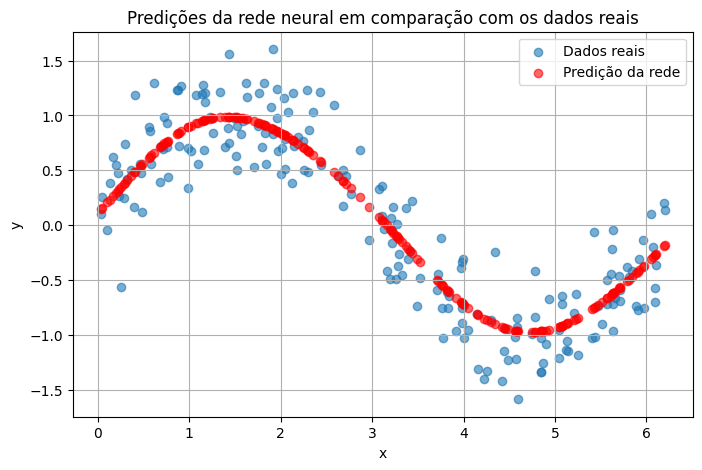
\includegraphics[width=\textwidth]{./0803_imgs/0365_tarefa05/png-241110-192954147-5354434943605266969.png}
		%		%\legend{Fonte: \citeonline[p. 24]{araujo2012}}
	\end{minipage}
	\hfill
	\begin{minipage}{0.45\textwidth}
		\centering
		\caption{$\sigma=0.5$}\label{fig:tarefa05:05:predicoes}
		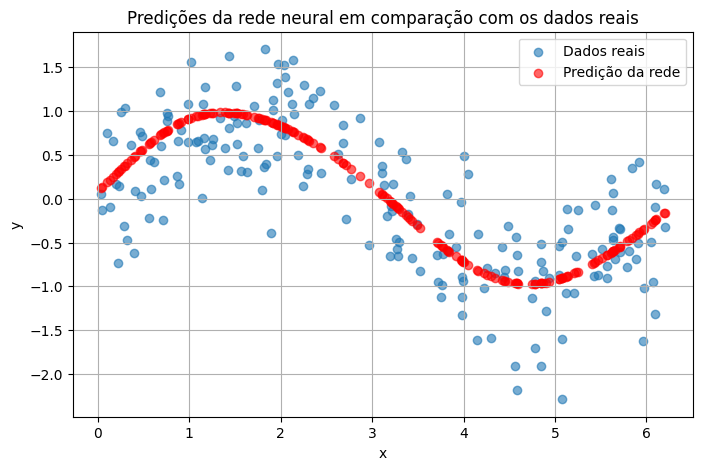
\includegraphics[width=\textwidth]{./0803_imgs/0365_tarefa05/png-241110-193141249-12530547749698557937.png}
		%\legend{Fonte: \citeonline[p. 24]{araujo2012}}
	\end{minipage}
\end{figure}



Em resumo, esta análise destaca a influência do ruído nos dados no processo de 
treinamento de modelos de aprendizado de máquina. Níveis mais altos de ruído 
podem levar a uma convergência mais lenta e instável, mas o modelo pode 
eventualmente adaptar-se e aprender a lidar com o ruído, como observado no caso 
de $\sigma=\num{0,5}$.